\documentclass[]{article}

\PassOptionsToPackage{numbers,compress}{natbib}

\usepackage[preprint]{neurips_2020_ml4ps}
\usepackage[utf8]{inputenc} 
\usepackage[T1]{fontenc}    
\usepackage{hyperref}       
\usepackage{url}            
\usepackage{booktabs}       
\usepackage{nicefrac}       
\usepackage{microtype}      
\usepackage{amsfonts,amsmath,amssymb}	
\usepackage{mathtools}
\usepackage{lipsum}
\usepackage[dvipsnames]{xcolor}

\definecolor{linkcolor}{rgb}{0.7752941176470588, 0.22078431372549023, 0.2262745098039215}
\hypersetup{colorlinks=true,
linkcolor=linkcolor,
citecolor=linkcolor,
urlcolor=linkcolor,
linktocpage=true,
pdfproducer=medialab,
}

\title{Inferring CDM substructure with \\ global astrometry beyond the power spectrum}

\author{
Siddharth Mishra-Sharma \\
Massachusetts Institute of Technology \\
The NSF AI Institute for Artificial Intelligence and Fundamental Interactions \\
New York University \\
\texttt{sm8383@nyu.edu} \\
}

\begin{document}

\maketitle

\begin{abstract}
\lipsum[2] 
\end{abstract}

\section{Introduction}
\label{sec:intro}

Although there exists plenty of evidence for dark matter (DM) on galactic scales and above,
% ---\emph{e.g.}, observations of galactic rotation curves, the physics of merging clusters, and the spectrum of fluctuations of the cosmic microwave background---
the DM distribution on sub-galactic scales is less well-understood and remains an active area of cosmological study. This distribution additionally correlates with and may provide clues as to the underlying particle physics nature of dark matter, highlighting its importance across multiple domains. 

While larger dark matter clumps---subhalos---can be detected and characterized through their association with luminous tracers like bound stellar populations, subhalos with smaller masses $\lesssim 10^9\,\mathrm M_\odot$ are not generally associated with luminous matter, rendering their characterization challenging. Gravitational effects thus provide one of the few avenues to probe the distribution of these otherwise invisible subhalos. Gravitational lensing \emph{i.e.}, the bending of light from a background source due to a foreground mass, is such an effect and has been proposed in various incarnations as a probe of the distribution of dark subhalos. Strong gravitational lensing, for example, has shown promise in probing substructure in galaxies outside of the Milky Way. \emph{Astrometric lensing} has on the other hand recently emerged as a powerful of the dark matter population in our own Galaxy.

\emph{Astrometry} refers to the precise measurement of the positions and motions of luminous objects like stars and other galaxies. Gravitational lensing of these background objects by a foreground mass, such as a dark matter subhalo, can imprint a characteristic pattern of motions on the measured kinematics (angular velocities and/or accelerations) of these objects. Ref.~\cite{VanTilburg:2018ykj} introduced several methods to extract this imprint with the aim of characterizing the subhalo population in our Galaxy, including methods based on computing convolutions of the expected induced lensing signal, detecting local kinematic outliers, and computing two-point correlators on the observed astrometric field. Ref.~\cite{Mishra-Sharma:2020ynk} further proposed using the power spectrum of the astrometric field as an observable to extract the properties of a dark matter population.

Astrometric datasets are inherently high-dimensional, consisting of positions and angular velocities and/or accelerations of potentially millions of objects. Especially when the signal consists of the collective imprint of a large number of dark matter objects, characterizing the properties of the population involves \emph{marginalizing} over all possible configurations of subhalos, rendering the likelihood intractable and necessitating a reduction to data summaries like the power spectrum. While shown to be effective, such simplification can result in loss of information when the signal is non-Gaussian in nature. Systematic effects such as the existence of large-scale power expressed in the low-dimensional summary domain can further inhibit signal sensitivity. 

The dawn of the era of precision astrometry, with the \emph{Gaia} satellite delivering the most precise astrometric dataset to-date and surveys including the Square Kilometer Array and Roman Space Telescope set to further change the game, calls for methods that can extract more information from these datasets than possible using existing techniques. In this paper we propose a method that leverages recent advances in simulation-based inference and neural network architectures in order to characterized the subhalo population in our Galaxy.



% First results~\cite{Mondino:2020rkn}
% Mining for substructure~\cite{Brehmer:2019jyt}

\section{Model and inference}
\label{sec:model}

\begin{figure}[!htbp]
\centering
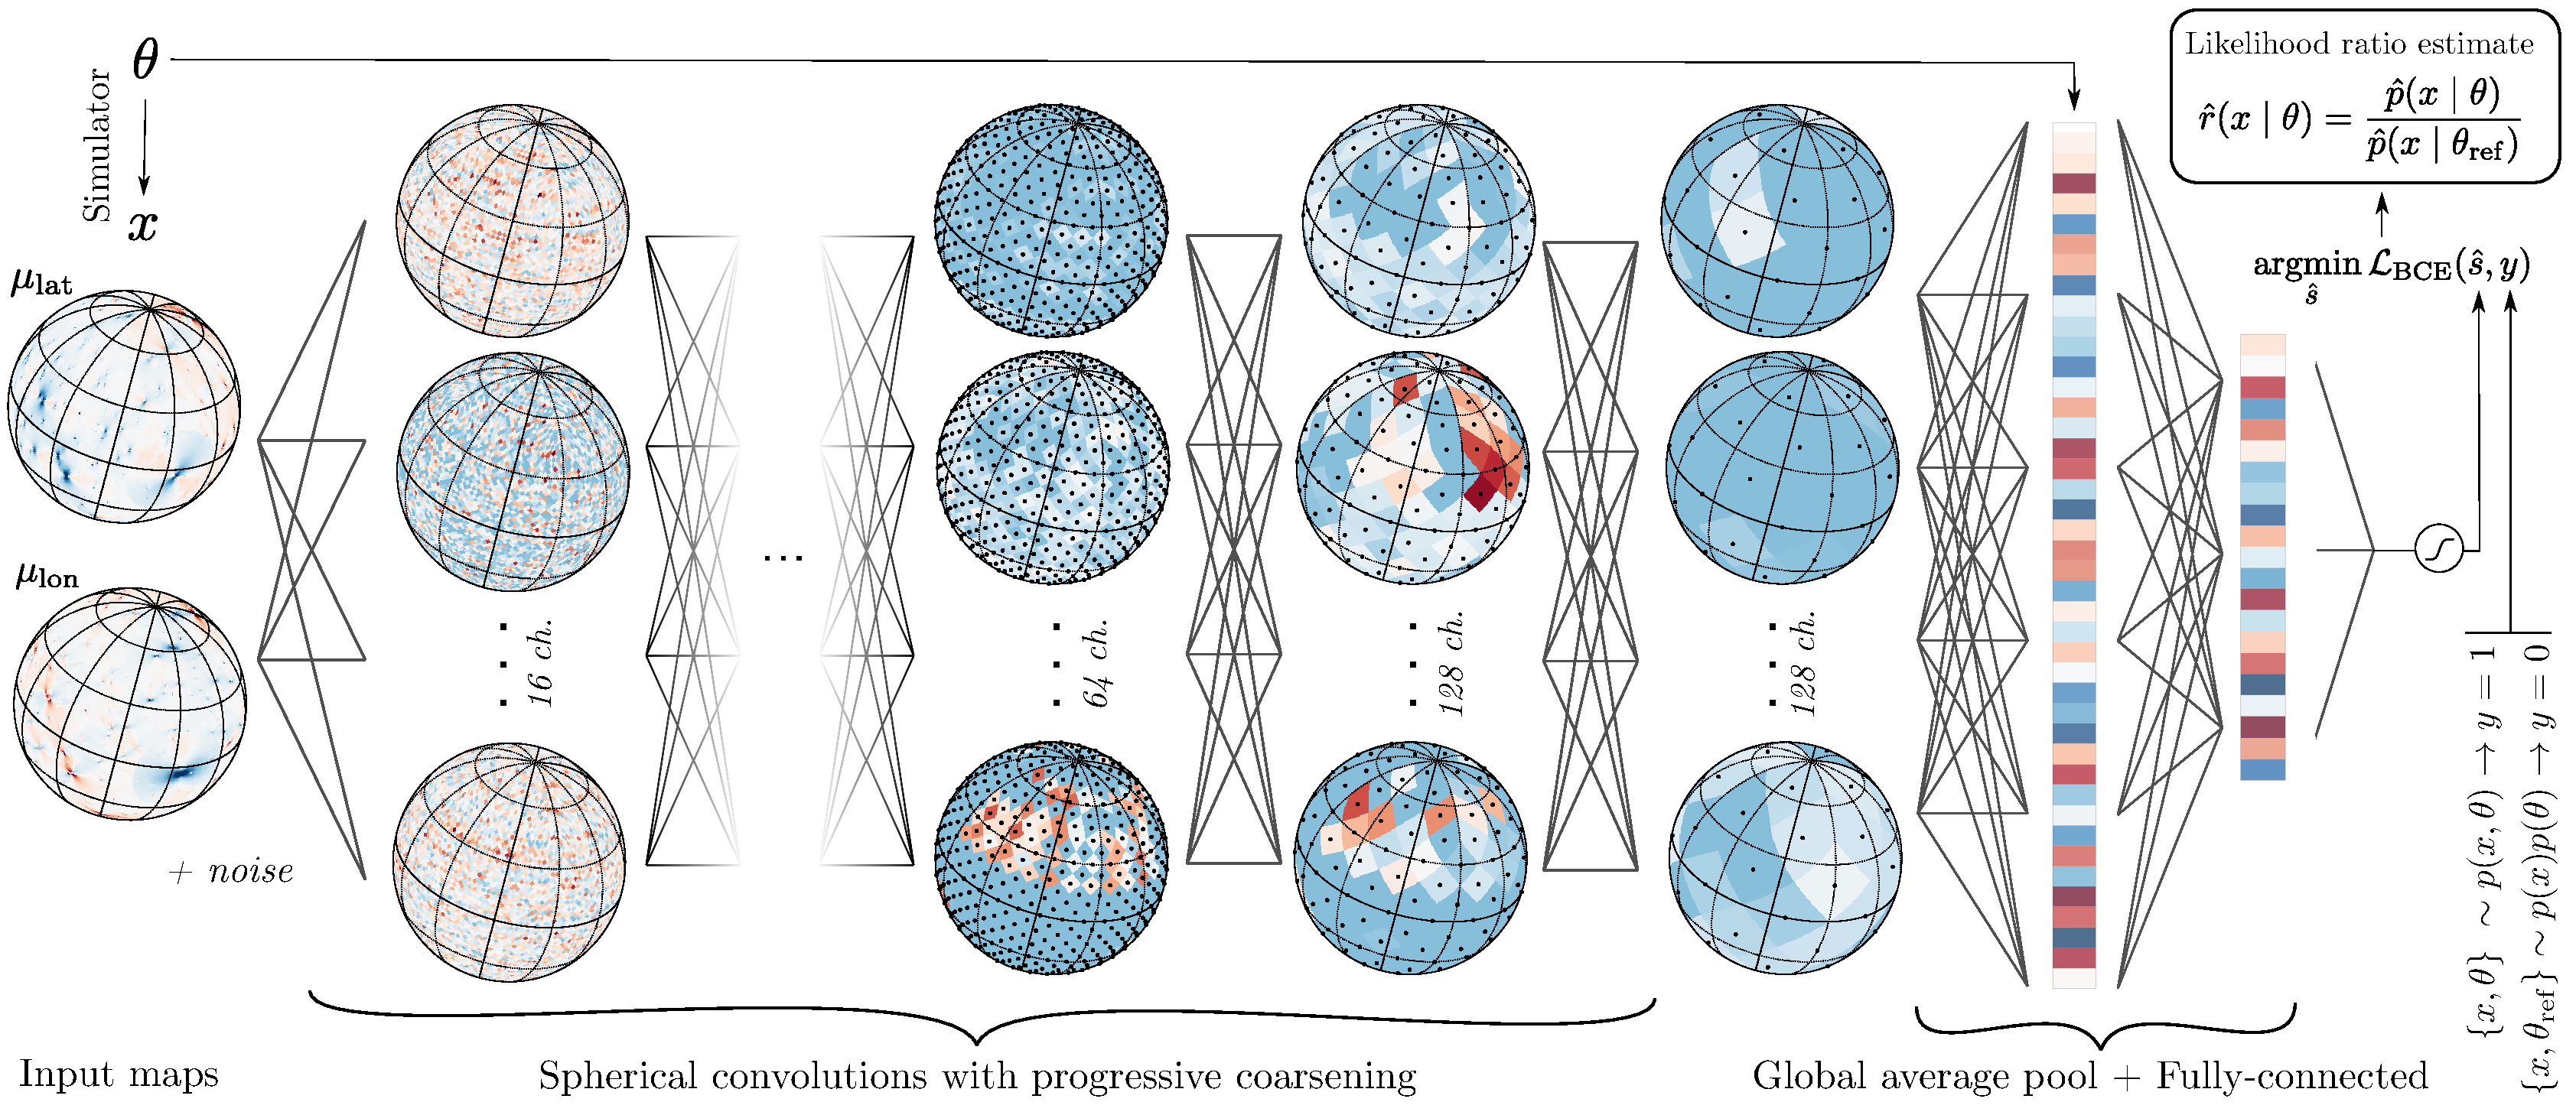
\includegraphics[width=0.98\textwidth]{figures/drawing.pdf}
\caption{Caption}
\label{fig:model}
\end{figure}

\paragraph{The forward model} We consider a population of Navarro-Frenk-White (NFW) subhalos following a power-law mass function, $\mathrm dn / \mathrm dm \propto m^\alpha$, with $\alpha = -1.9$ as expected if the population is sources from a nearly scale-invariant distribution of primordial fluctuations in the $\Lambda$CDM scenario. 
% Subhalos between $10^7$--$10^{10}\,\mathrm{M}_\odot$ are simulated. 
The subhalo fraction $f_\mathrm{sub}$, quantifying the expected fraction of the mass of the Milky Way contributed by subhalos in the mass range $10^{-6}$--$10^{10}\,\mathrm{M}_\odot$, is taken to be the parameter of interest. The fiducial scenario is taken to contain 150 subhalos in expectation between $10^{8}$--$10^{10}\,\mathrm{M}_\odot$, corresponding to $f_\mathrm{sub} \simeq 0.2$ and motivated by results from the Aquarius simulation. The spatial distribution of subhalos is again modeled using results from the Aquarius simulation, following Ref.~\cite{}.

Our dataset consists of the 2-dimensional velocity map of quasi-stellar objects (QSOs), also known as quasars which, owing to their large distances from us, are expected to have small intrinsic proper motions. We assume the velocity maps are discretized on a \texttt{HEALPix} grid with resolution parameter \texttt{nside=64}, the value in each pixel then quantifying the average velocity of quasars within that pixel. Given a subhalo with velocity $\mathbf{v}_{l}$, the expected induced velocity in a given pixel is
\begin{equation}
    \boldsymbol{\mu}(\mathbf{b})=4 G_{\mathrm{N}}\left\{\frac{M(b)}{b^{2}}\left[2 \hat{\mathbf{b}}\left(\hat{\mathbf{b}} \cdot \mathbf{v}_{l}\right)-\mathbf{v}_{l}\right]-\frac{M^{\prime}(b)}{b} \hat{\mathbf{b}}\left(\hat{\mathbf{b}} \cdot \mathbf{v}_{l}\right)\right\}
\end{equation}
where $M(b)$ and $M^{\prime}(b)$ are the projected mass and its gradient at impact parameter $\mathbf{b}$, given by the vector between the centers of the subhalo and pixel. An example of part of the induced velocity signal map on the celestial sphere, projected along the latitudinal and longitudinal directions, is shown in the leftmost column of Fig.~\ref{fig:model}.

In order to enable comparison with traditional approaches---which are generally not expected to be sensitive to a CDM subhalo population with next-generation astrometric surveys---we use an optimistic observational configuration corresponding to measure the proper velocities of $10^9$ quasars with expected noise $\sigma_{\mu} = 0.1\,\mu\mathrm{as}\,\mathrm{yr}^{-1}$.

\paragraph{The power spectrum approach} Ref.~\cite{Mishra-Sharma:2020ynk} introduced an approach for extracting the astrometric signal due to a dark matter population by decomposing the observed map into its \emph{angular power spectrum}. The power spectrum is a summary statistic ubiquitous in astrophysics and cosmology, and quantifies the amount of correlation contained across different scales. In the case of data on a sphere, the basis of spherical harmonics is often used, and the power spectrum then encodes the correlation structure on different multipoles $\ell$. The power spectrum effectively captures the \emph{linear} component of the signal and, when the underlying signal is a Gaussian random field (exemplified by the Cosmic Microwave Background), captures all of the relevant information contained in the map(s).

The expected signal in the power spectrum domain can be computed analytically using the formalism described in Ref.~\cite{Mishra-Sharma:2020ynk}, which we use here as a comparison point. While effective, reduction of the full astrometric map to its power spectrum results in loss of information; this can be seen from the fact that the signal on the leftmost column of Fig.~\ref{fig:model} is far from Gaussian. Furthermore, the existence of systematic, unaccounted-for correlations on large angular scales (as measure on data from the \emph{Gaia} satellite in Refs.~\cite{}) introduced degeneracies with a putative signal and precludes their usage in the present context. This is especially true when \emph{relative} astrometry is employed, and systematic variations between observed patches of the sky are present. For this reason multipoles $\ell < 10$ were discarded in Ref.~\cite{Mishra-Sharma:2020ynk}, degrading the projected sensitivity.

\paragraph{Simulation-based inference with parameterized classifiers} Recent advances in machine learning have enabled methods that aim to directly extract information from models defined through high-dimensional simulations; see Ref.~\cite{Cranmer:2019eaq} for a recent review. Here, we make use of parameterized classifiers in order to approximate the likelihood ratio associated with all-sky astrometric maps containing signatures of dark matter. Given a classifier that can distinguish between samples $x \sim p(x\mid\theta)$ and those from a fixed reference hypothesis $x \sim p(x\mid\theta_\mathrm{ref})$, the decision function output by the optimal classifier $s(x, \theta) = \frac{p(x\mid\theta)}{p(x\mid\theta) + p(x\mid\theta_\mathrm{ref})}$ is one-to-one with the likelihood ratio, $r(x\mid \theta) \equiv \frac{p(x\mid\theta)}{p(x\mid\theta_\mathrm{ref})}  = \frac{s(x, \theta)}{1 - s(x, \theta)}$. 

The classifier $d(x, \theta)$ in this case is a neural network that can work directly on the high-dimensional data $x$, and is parameterized by $\theta$ by including it as a feature in the neural network. In order to improve numerical stability and reduce dependence on the fixed reference hypothesis $\theta_\mathrm{ref}$, we follow Refs.~\cite{} and train a classifier to distinguish between data-sample pairs $\{x, \theta\} \sim p(x,\theta)$ and those from the marginal model $\{x, \theta\} \sim p(x)p(\theta)$ using the binary cross-entropy loss as the optimization objective. 

\paragraph{Extracting information from high-dimensional datasets} Out input dataset consists of a two-component velocity vector uniformly sampled on the sphere following the \texttt{HEALPix} representation. We use \texttt{DeepSphere}, a graph-based convolutional neural network (CNN) architecture tailored to data sampled on a sphere, and is able to leverage the hierarchical structure of the \texttt{HEALPix} representation. In particular, \texttt{DeepSphere} efficiently performs convolutions in the spectral domain, using a basis of Chebychev polynomials as the convolutional kernels. 

Starting with 2 input channels representing the two orthogonal components of the velocity vector at resolution \texttt{nside=64}, we perform a graph convolution operation, increasing the channel dimension to 16, following by a batch normalization, ReLU nonlinearity, and a max pooling operation to coarsen the resolution to \texttt{nside=32}. Four more such convolutional layers are employed, increasing the channel by a factor of 2 at each step until a maximum of 128, with the final map having \texttt{nside=2}. At this stage, we average over the spatial dimension in order to encourage feature rotational invariance, outputting 128 features to which the parameter of interest $f_\mathrm{sub}$ is appended. This is passed through a fully-connected network with (1024, 128) hidden units outputting the classifier decision by applying a sigmoidal projection.

$10^5$ samples from the forward model are produced, and the parameterized likelihood-ratio estimator is trained for 50 epochs using the \texttt{AdamW} optimizer with initial learning rate $10^{-3}$ and weight decay $10^{-5}$.

% LRT~\cite{Cranmer:2015bka}
% AALR~\cite{Hermans:2019ioj}
% SBI~\cite{Cranmer:2019eaq}

\begin{figure}[!htbp]
\centering
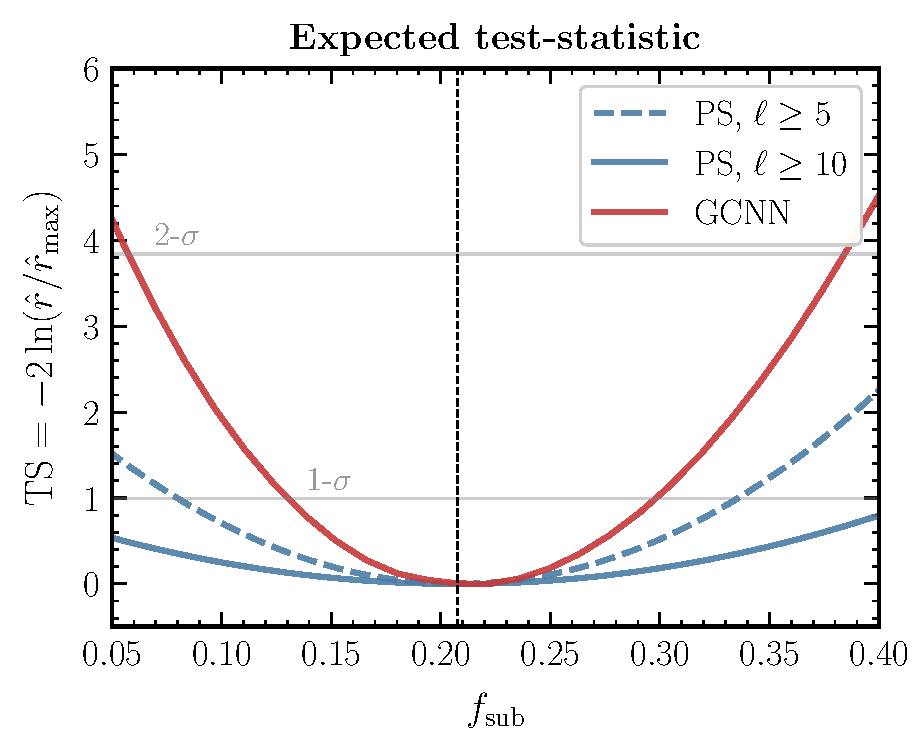
\includegraphics[width=0.49\textwidth]{figures/TS}
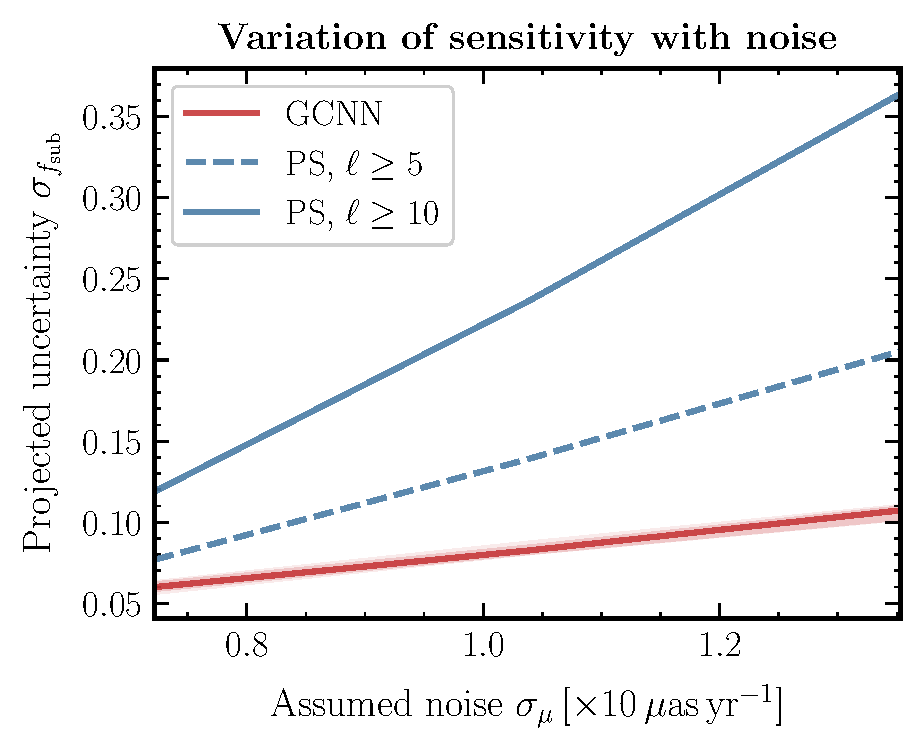
\includegraphics[width=0.49\textwidth]{figures/noise_var}
\caption{Caption}
\label{fig:experiment}
\end{figure}
 
% \begin{figure}[!htbp]
% \centering
% 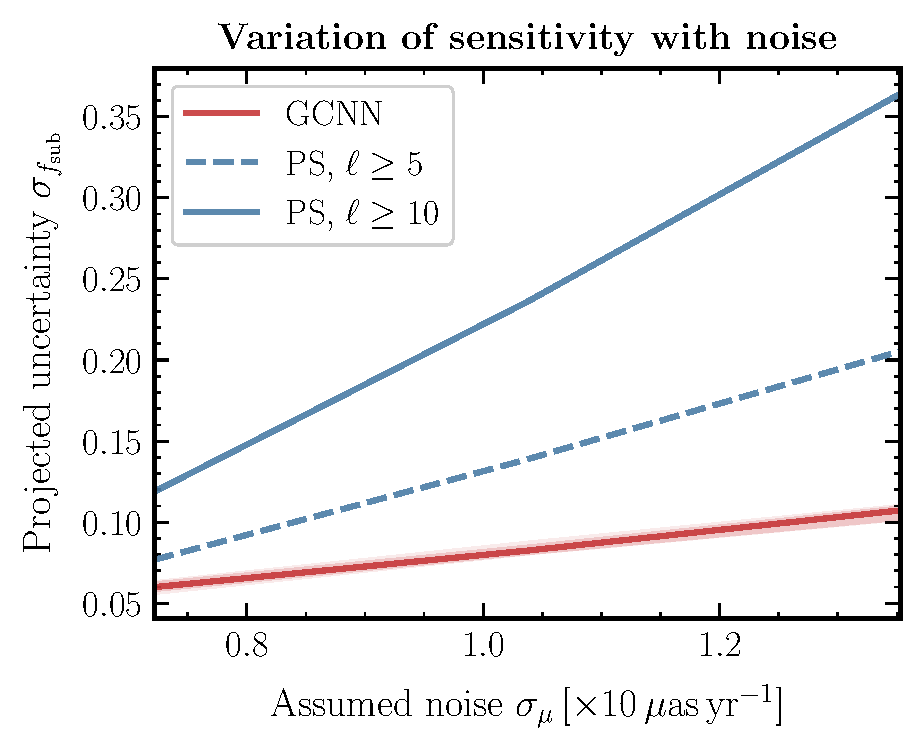
\includegraphics[width=0.49\textwidth]{figures/noise_var}
% \caption{Caption}
% \label{fig:experiment}
% \end{figure}

\section{Results on simulated data}
\label{sec:experiments}

The left panel of Fig.~\ref{fig:experiment} shows the expected test statistic (TS), defined as $\mathrm{TS} \equiv -2\ln(\hat r / \hat r_\mathrm{max})$, as a function of substructure fraction $f_\mathrm{sub}$ evaluated on test maps of the fiducial signal with $f_\mathrm{sub} \simeq 0.2$. Corresponding curves using the power spectrum approach are shown in blue, using minimum multipole thresholds of $\ell = 5$ (dashed) and $\ell = 10$ (solid). Thresholds corresponding to 1- and 2-$\sigma$ discovery are shown as the horizontal grey lines. We see that sensitivity gains of over a factor of $\sim 2$ can be expected when using the machine learning approach presented here when compared to the traditional power spectrum approach. 

The right panel of Fig.~\ref{fig:experiment} shows the scaling of expected sensitivity on substructure fraction $f_\mathrm{sub}$ with assumed noise per quasar, keeping the number of quasars fixed (red band, showing 1-$\sigma$ variation over test datasets) compared to the power spectrum approach (blue lines). A far more favorable scaling of the machine learning approach is seen compared to the power spectrum approach, suggesting that it may be disproportionately advantageous in the low signal-to-noise regimes that are generally most relevant for dark matter searches.

\section{Conclusions and outlook}
\label{sec:conclusions}

In this paper we have leveraged recent advances in simulation-based inference and neural network architectures in order to introduce a method to analyze astrometric datasets over large regions of the sky, with the aim of inferring the signatures 

\begin{enumerate}
    \item Population hasn't been observed
    \item Data is expensive
    \item Break degeneracies
    \item Use of more complex architectures
    \item Other scenarios and the acceleration spectrum, smaller FOV
\end{enumerate}

Code and data used for reproducing the results presented in this paper is available at \url{https://github.com/smsharma/sbi-astrometry}.

\section*{Broader Impact}
\label{sec:impact}

% Accounting for epistemic uncertainty is crucial for making robust conclusions from data in machine learning applications. This work is part of the broader scientific effort to design and implement techniques that attempt to incorporate deficiencies in our ability to model consequential aspects of real-world data in a principled manner.

We acknowledge the importance of considering the ethical implications of scientific research in general, and machine learning research in particular, as well as of placing both the process and output of scientific research in a broader societal context. We do not believe the present work presents any issues in this regard. 

\begin{ack}
SM would like to thank the Center for Computational Astrophysics at the Flatiron Institute for their hospitality while this work was being performed. 
This work was performed in part at the Aspen Center for Physics, which is supported by National Science Foundation grant PHY-1607611.
The participation of SM at the Aspen Center for Physics was supported by the Simons Foundation.
SM is supported by the NSF CAREER grant PHY-1554858, NSF grants PHY-1620727 and PHY-1915409, and the Simons Foundation. 
This work made use of the NYU IT High Performance Computing resources, services, and staff expertise. 
This research has made use of NASA's Astrophysics Data System. 
This research made use of the Astropy~\cite{Robitaille:2013mpa,Price-Whelan:2018hus},
\texttt{HEALPix}~\cite{Gorski:2004by,Zonca2019},
IPython~\cite{PER-GRA:2007},
Jupyter~\cite{Kluyver2016JupyterN},
Matplotlib~\cite{Hunter:2007},
NumPy~\cite{harris_array_2020},
Pyro~\cite{bingham2019pyro},
PyTorch~\cite{NEURIPS2019_9015},
SciPy~\cite{2020SciPy-NMeth}, and
Seaborn~\cite{michael_waskom_2017_883859}
software packages.
\end{ack}

\bibliographystyle{apsrev4-1-mod}
\bibliography{sbi-astrometry}

\end{document}